
\documentclass[10pt]{article}
\usepackage[utf8]{inputenc}
\usepackage{kotex}
\usepackage{graphicx}
\usepackage{subfigure}
\usepackage{titling}
\setlength{\droptitle}{-2cm}
\usepackage{array}
\usepackage{amssymb}
\usepackage{amsmath}
\usepackage{siunitx} 
\usepackage{enumerate} 
\usepackage{pgfplots}
\usepackage{pgfplotstable}
\usepackage{tikz,pgfplots}
\usepackage{wasysym}
\usepackage{geometry}
\usepackage{authblk}
\usepackage{kotex}
\usepackage{bibunits}
\usepackage{tabularx}
\usepackage{hyperref}
\usepackage{pythonhighlight}

\geometry{
    a4paper,
    total={170mm,257mm},
    left=20mm,
    top=20mm,
}

\title{\textbf{Mathematical Foundation of DNN : HW 1}}
\author{Jeong Min Lee}

\begin{document}
\maketitle
\section*{Notations}
\begin{enumerate}
    \item $\otimes$ : convolution
    \item $v^{(i)}$ : $i$th element of vector $v\in \mathbb{R}^n$
    \item $A^{(i,j)}$ : the element of matrix $A\in \mathbb{R}^{m\times n}$ in $i$th row and $j$th column 
    \item $\delta_{ij}$ : Kronecker delta symbol.
\end{enumerate}
\section{}
Let $\omega^{(1)}, \omega^{(2)}\in\mathbb{R}^{3 \times 3}$ denote the map from $X$ to $Y_1, Y_2$, respectively. Then, 
$\omega \in \mathbb{R}^{(2\times 3 \times 3)} = [\omega^{(1)}, \omega^{(2)}]$.
Noting that the process of discrete convolution and being aware of where the filter maps each image pixel $X_{ij}$, 
$\omega^{(1)},\omega^{(2)}$ can be represented as follow.

\begin{equation}
    \omega^{(1)} = \begin{pmatrix}
        0 & 0 & 0 \\ 0 & -1 & 0 \\ 0 & 1 & 0
    \end{pmatrix}
\end{equation}

\begin{equation}
    \omega^{(2)} = \begin{pmatrix}
        0 & 0 & 0 \\ 0 & -1 & 1 \\ 0 & 0 & 0
    \end{pmatrix}
\end{equation}

For instance,
\begin{equation*}
    \begin{pmatrix}
        X_{11} & X_{12} & X_{13} \\ X_{21} & X_{22} & X_{23} \\ X_{31} & X_{32} & X_{33}
    \end{pmatrix}
    \otimes 
    \begin{pmatrix}
        0 & 0 & 0 \\ 0 & -1 & 0 \\ 0 & 1 & 0
    \end{pmatrix}
    = X_{32} - X_{22} = Y_{22}
\end{equation*}

\section{}
We can formalized this problem as following example.
\begin{equation*}
    \begin{pmatrix}
        a & b & c \\ d & e & f \\ g & h & i
    \end{pmatrix}
    \otimes
    \begin{pmatrix}
        \empty & \empty & \empty \\ \empty & ? & \empty \\ \empty & \empty & \empty
    \end{pmatrix}
    = \frac{1}{9}(a + b + c + d + e + f + g + h + i)
\end{equation*}
This is obvious that $I_k/k^2$ satisfy the condition above, where $I_k$ is $k$ dimensional identity matrix.
Note that we have to divide all summation of subimage since there are $k^2$ pixels that overlap with the filter whose size is $k$.

\section{}
This problem is obvious that $\omega = [0.299, 0.587, 0.114]\in\mathbb{R}^{3\times 1 \times 1}$. 
As the given expression $Y_{ij} = 0.299X_{1,i,j} + 0.587 X_{2,i,j} + 0.114 X_{3,i,j}$ says, $1\times 1$ convolution is a type of constant multiplicatioon for each channel.
The reason we use $1\times 1$ convolution can be elucidated by seeing the following example: Consider the 192 gray scale images $X \in \mathbb{R}^{192\times 28 \times 28}$. Doing appropriate padding to conserve the output dimension, using a filter whose size is $5$ and channel is $32$ returns $32 \times 28 \times 28$ activation maps. 
The number of float multiplication calculation in this case is $28\times 28\times 32 \times 5 \times 192 = 120$M. However, inserting 1d convolution whose depth is 16 results in the activation map whose dimension is $16 \times 28 \times 28$.(Again, I assumed appropriate padding to preserve the dimension.) Then, applying $32\times 5 \times 5$ makes the output activation map have $32 \times 28 \times 28$ dimension. (Note that this secondary filter is identical to the filter in the first case.)
For second case, the number of computations is $28\times 28 \times 1 \times 1\times 192 + 28\times 28\times 32 \times 5 \times 5 \times 16 = 12.4$M, which is 10 times smaller than the first case.  
This example implies that inserting 1d convolution between the filter convolving the image reduces the time complexity of the model and can improve the model's performance.

\section{}
\textbf{CLAIM : }$\sigma$ can commute to $\max$
\\
\textbf{proof : }
Consider $S = \left\{a_1,a_2,\cdots, a_n\right\}\in\mathbb{R}^n$. Withoug loss of generality, suppose $\max S = a_1$. Then, $\sigma(\max S) = \sigma(a_1)$. 
However, noting that $\sigma$ is non-decreasing function, $\max\left\{\sigma(a_1), \cdots,\sigma(a_n) \right\} = \sigma(a_1)$. Otherwise, there is some $a_i \in S\backslash\left\{a_1\right\}$ s.t. $\sigma(a_i) > \sigma(a_1)$. However, since $a_i\le a_1$, it contradicts to the non-decreasing assumption of $\sigma$.
Thus, $\sigma$ and $\max$ commute each other.$\blacksquare$

Let $\mathfrak{M}_{m,n}(F)$ be the set of $m\times n$ matrices over some field $F$. Then, in alegebra, it is well known fact that $\mathfrak{M}_{m,n}(F)$ is isomorphic to $F^{mn}$.\footnote{This is corollary of the following theorem : $V \approx W \iff \text{dim}V = \text{dim}W$ for two vector spaces $V, W$.}
Letting $F = \mathbb{R}$, one can apply the \textbf{CLAIM} to the $X\in\mathfrak{M}_{m,n}(\mathbb{R})$.
Since $\rho$ maps from $\mathbb{R}^{m\times n}$ to $\mathbb{R}^{k\times l}$, the filter size that $\rho$ uses is $(m/k, n/l)$. 
Considering the feature of max pooling, $\rho = \max$ for the input whose size is identical to the filter size. 
Let's denote
\begin{equation*}
    X_{i:i+m/k-1, j:j+n/l-1} = \begin{pmatrix}
        X_{ij} & \cdots & X_{i,j+n/l-1} \\ \vdots & \ddots & \vdots \\ X_{i+m/k-1,j} & \cdots & X_{i+m/k-1,j+n/l-1}
    \end{pmatrix}
\end{equation*}
and $y_{ij} = \max X_{i:i+m/k-1,j:j+n/l-1}$. Then, $\rho(X) = (y_{ij})$. 
\begin{align*}
    \sigma(\rho(X_{i:i+m/k-1,j:j+n/l-1})) &= \sigma\left(\max \begin{pmatrix}X_{ij} & \cdots & X_{i,j+n/l-1} \\ \vdots & \ddots & \vdots \\ X_{i+m/k-1,j} & \cdots & X_{i+m/k-1,j+n/l-1} \end{pmatrix}\right)
    \\ &= \max \left(\begin{pmatrix}
        \sigma(X_{ij}) & \cdots & \sigma(X_{i,j+n/l-1}) \\ \vdots & \ddots & \vdots \\ \sigma(X_{i+m/k-1,j}) & \cdots & \sigma(X_{i+m/k-1,j+n/l-1})
    \end{pmatrix}\right)
    \\ &= \rho(\sigma(X_{i:i+m/k-1,j:j+n/l-1}))
    \\ &= \sigma(y_{ij})
\end{align*}
This implies that $\sigma$ and $\rho$ can commute.

\section{}
To solve this problem, I refered the Chapter 2 code in the lecture. Please see appendix to get my implementations.
Comparing the test result of two implementations, using KL-divergence and MSE loss, it was revealed that their performances are similar. 
To elucidate the reason using the KL-divergence rather than MSE in several vision tasks, I performed multiple times of training and testing. Furthermore, I recorded the time consumed by training and testing.
See the table below.

\begin{table}[!h]
    \begin{center}
        \begin{tabular}{lllll}
            & \multicolumn{2}{c}{$D_{KL}$} \vline & \multicolumn{2}{c}{MSE} \\
            \hline \hline
            & Accuracy(\%)    & Time(s)         & Accuracy(\%)  & Time(s)        \\
    1       & 92.16       & 2.8         & 95.58     & 6.4         \\
    2       & 96.63       & 2.8         & 95.38     & 6.4         \\
    3       & 95.98       & 3.0           & 95.28     & 6.3         \\
    4       & 96.08       & 2.8         & 94.98     & 6.5         \\
    5       & 96.84       & 2.8         & 88.15     & 6.4         \\
    \hline 
    average & 95.538      & 2.84        & 93.874    & 6.4         \\
    std     & 1.71974882  & 0.08 & 2.86854388      & 0.06324555 
    \end{tabular}
    \end{center}
    \caption{The performace test of MSE loss and KL-divergence loss($D_{KL}$)}
    \label{tab1}
\end{table}
As Table \ref{tab1} says, the overal accuary of $D_{KL}$ is slightly higher than MSE($95.538\% > 93.874\%$).
Furthermore, as the standard deviation of accuracies says, $D_{KL}$ is more stable than MSE($1.720< 2.869$). 
Finally, the training and testing time of $D_{KL}$ is much less than that of MSE. I thinks that this results from the computation of square in MSE. In general, the computation of power in floating numbers is slow in python.
Considering that accuracy and computation time complexity are crucial aspects for the DL algorithms, implementation using $D_{KL}$ loss is more choosable. 


\section{}
\subsection*{(a)}
Note that $y_L,b_L\in \mathbb{R}$ and $A_L \in \mathbb{R}^{1\times n_{L-1}}$
\subsubsection*{(i)}
\begin{equation*}
    {\partial y_L \over \partial b_L}  = {\partial b_L \over \partial b_L} = 1
\end{equation*}
\subsubsection*{(ii)}
From $A_Ly_{L-1} = A_L^{(1)}y_{L-1}^{(1)} + \cdots + A_L^{(n_{L-1})}y_{L-1}^{(n_{L-1})}$
\begin{align*}
    {\partial y_L \over \partial y_{L-1}} &= {\partial A_L y_{L-1} \over y_{L-1}} \\
    &= \left({\partial A_Ly_{L-1} \over \partial y_{L-1}^{(1)}}, \cdots, {\partial A_Ly_{L-1} \over \partial y_{L-1}^{(n_{L-1})}}\right) \\
    &= \left(A_L^{(1)},\cdots, A_L^{(n_{L-1})}\right)\\
    &= A_L
\end{align*}
\subsubsection*{(iii)}
Let $z_l = A_l y_{l-1} + b_l$.Then,
\begin{align*}
    {\partial y_l \over \partial b_l} &= {\partial \sigma(z_l) \over \partial b_l} \\
    &= \begin{pmatrix}
        {\partial \sigma(z_l^{(1)}) \over \partial b_l^{(1)}} & \cdots & {\partial \sigma(z_l^{(1)}) \over \partial b_l^{(n_l)}}\\
        \vdots & \ddots & \vdots \\
        {\partial \sigma(z_l^{(n_l)}) \over \partial b_l^{(1)}} & \cdots & {\partial \sigma(z_l^{(n_l)}) \over \partial b_l^{(n_l)}}
    \end{pmatrix}\\ \\
    {\partial \sigma(z_l^{(i)}) \over \partial b_l^{(j)}} &= \sigma^\prime(z_l^{(i)}) {\partial z_l^{(i)} \over \partial b_l^{(j)}} \\
    &= \sigma^\prime(z_l^{(i)}) \delta_{ij}\\ \\
    \therefore {\partial y_l \over \partial b_l} &= \begin{pmatrix}
        \sigma^\prime(z_l^{(1)}) & \cdots & 0 \\
        \vdots & \ddots & \vdots \\
        0 & \cdots & \sigma^\prime(z_l^{(n_l)})
    \end{pmatrix} = \text{diag}(\sigma^{\prime}(A_ly_l + b_l))
\end{align*}
\subsubsection*{(iv)}
\begin{align*}
    {\partial y_l \over \partial y_{l-1}} &= {\partial \sigma(z_l) \over \partial y_{l-1}} \\
    &= \begin{pmatrix}
        {\partial \sigma(z_l^{(1)}) \over \partial y_{l-1}^{(1)}} & \cdots & {\partial \sigma(z_l^{(1)}) \over \partial y_{l-1}^{(n_{l-1})}}\\
        \vdots & \ddots & \vdots \\
        {\partial \sigma(z_l^{(n_l)}) \over \partial y_{l-1}^{(1)}} & \cdots & {\partial \sigma(z_l^{(n_l)}) \over \partial y_{l-1}^{(n_{l-1})}}
    \end{pmatrix}\\ \\
    {\partial \sigma(z_l^{(i)}) \over \partial y_{l-1}^{(j)}} &= \sigma^\prime(z_l^{(i)}) {\partial z_l^{(i)} \over \partial y_{l-1}^{(j)}}
    = \sigma^\prime(z_l^{(i)}) A_l^{(i,j)}\quad \left(\because z_l^{(k)} = \sum_p A_l^{(k,p)}y_{l-1}^{(p)} + b_l^{(k)}\right)\\ \\
    \therefore {\partial y_l \over \partial y_{l-1}} &= \begin{pmatrix}
        \sigma^\prime(z_l^{(1)})A_l^{(1,1)} & \cdots & \sigma^\prime(z_l^{(1)})A_l^{(1,n_{l-1})} \\
        \vdots & \ddots & \vdots \\
        \sigma^\prime(z_l^{(1)})A_l^{(n_l,1)} & \cdots & \sigma^\prime(z_l^{(1)})A_l^{(n_l,n_{l-1})}
    \end{pmatrix}\\
    &= \text{diag}(\sigma^{\prime}(A_ly_l + b_l))A_l
\end{align*}

\subsection*{(b)}
\subsubsection*{(i)}
\begin{equation*}
    {\partial y_L \over \partial A_L} = {\partial A_Ly_{L-1} \over \partial A_L} = \left({\partial \over A_L^{(1)}}A_Ly_{L-1}, \cdots, {\partial \over A_L^{(n_{L-1})}}A_Ly_{L-1}\right) = y_{L-1}^T
\end{equation*}

\subsubsection*{(ii)}
To prove ${\partial y_L \over \partial A_l} = \text{diag}(\sigma^\prime(A_ly_{l-1} + b_l))\left({\partial y_L \over \partial y_l}\right)^Ty_{l-1}^T$.
it is enough to show the following, introducing $z_l = A_ly_{l-1} + b_l$.

\begin{equation}
    {\partial y_L \over \partial A_l^{(i,j)}} = \sigma^\prime(z_l^{(i)}){\partial y_L \over \partial y_l^{(i)}} y_{l-1}^{(j)}
\end{equation}
To show the above relation, consider the chain rule. 
\begin{equation*}
    {\partial y_L \over \partial A_l^{(i,j)}} = {\partial y_L \over \partial y_l} {\partial y_l \over \partial A_l^{(i,j)}} \\ 
\end{equation*}
Then, calculate both terms as follow.
\begin{align*}
    {\partial y_l \over \partial A_l^{(i,j)}} &= \left({\partial \sigma(z_l^{(1)}) \over \partial A_l^{(i,j)}}, \cdots, {\partial \sigma(z_l^{(n_l)}) \over \partial A_l^{(i,j)}}\right)^T \\
    {\partial \sigma(z_l^{(k)}) \over \partial A_l^{(i,j)}} &= \sigma^\prime(z_l^{(k)}){\partial z_l^{(k)}\over \partial A_l^{(i,j)}} = \sigma^\prime(z_l^{(k)})\delta_{ik}y_{l-1}^{(j)} \quad \left(\because z_l^{(k)} = \sum_p A_l^{(k,p)}y_{l-1}^{(p)}+ b_l^{(k)}\right)\\
    \therefore {\partial y_l \over \partial A_l^{(i,j)}} &= \left(0, \cdots, \sigma^\prime(z_l^{(i)})y_{l-1}^{(j)}, \cdots, 0 \right)^T
\end{align*}
Note that the nonzero element is located at the $i$th position. Then, since ${\partial y_L\over \partial y_l} = \left({\partial y_L\over \partial y_l^{(1)}}, \cdots, {\partial y_L\over \partial y_l^{(n_l)}}\right)$,
\begin{equation*}
    {\partial y_L\over \partial A_l^{(i,j)}} = \left({\partial y_L\over \partial y_l^{(1)}}, \cdots, {\partial y_L\over \partial y_l^{(n_l)}}\right) \cdot \left(0, \cdots, \sigma^\prime(z_l^{(i)})y_{l-1}^{(j)}, \cdots, 0 \right)^T = \sigma^\prime(z_l^{(i)}){\partial y_L \over \partial y_l^{(i)}} y_{l-1}^{(j)}
\end{equation*}

\section{}
The following is the code I implemented to solve this problem. Using the following code, the test accuracy for original LeNet5 was about 98.64\%, while that for mordern LeNet5 was 98.71\%
The time consumed to train and test original LeNet5 was 18m 41sec, while mordern LeNet5 was 2m 42sec. 
Eventhough two algorithms have similar performance, the time complexity to train original LeNet5 takes approximately 10 time longer time. This is because $C_3$ layer in original LeNet5 is much more complex than that in mordern LeNet5.

Next, discussing the trainable parameters of both algorithms is meaningful. The only difference of original LeNet5 and mordern one is the $C_3$ layer. Thus, the difference of trainable parameters must be equal to that of $C_3$ layer. 
The number of trainable parameter of original LeNet5 was 60806, while that of mordern LeNet5 was 61706. According to the following calculation, the number of trainable parameters of original LeNet5 was 1516, while that of mordern LeNet5 was 2416.
\begin{equation*}
    6\times (5\times5\times3 + 1) + 9\times(5\times5\times4+1) + 1\times(5\times5\times6 + 1)
\end{equation*}
The difference of the number of trainable parameters between original LeNet5 and mordern one was 900, which agrees to the difference between the total trainable parameters of original LeNet5 and mordern one.
Thus, the handwritten computation matches to the result of the code. 

\begin{figure}[!h]
    \begin{center}
        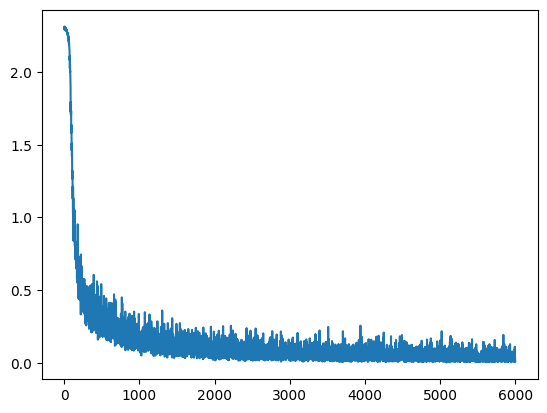
\includegraphics[scale = 0.5]{figure/fig1.png}
    \end{center}
    \caption{The training loss of problem 7 for each iteration.}
\end{figure}
\begin{python}
import torch
import torch.nn as nn
from torch.optim import Optimizer
from torch.utils.data import DataLoader
from torchvision import datasets
from torchvision.transforms import transforms
import matplotlib.pyplot as plt 

device = torch.device("cuda" if torch.cuda.is_available() else "cpu")

'''
Step 1:
'''

# MNIST dataset
train_dataset = datasets.MNIST(root='./mnist_data/',
                               train=True, 
                               transform=transforms.ToTensor(),
                               download=True)

test_dataset = datasets.MNIST(root='./mnist_data/',
                              train=False, 
                              transform=transforms.ToTensor())


'''
Step 2: LeNet5
'''

# Modern LeNet uses this layer for C3
class C3_layer_full(nn.Module):
    def __init__(self):
        super(C3_layer_full, self).__init__()
        self.conv_layer = nn.Conv2d(6, 16, kernel_size=5)

    def forward(self, x):
        return self.conv_layer(x)

# Original LeNet uses this layer for C3
class C3_layer(nn.Module):
    def __init__(self):
        super(C3_layer, self).__init__()
        self.ch_in_3 = [[0, 1, 2],
                        [1, 2, 3],
                        [2, 3, 4],
                        [3, 4, 5],
                        [0, 4, 5],
                        [0, 1, 5]] # filter with 3 subset of input channels
        self.ch_in_4 = [[0, 1, 2, 3],
                        [1, 2, 3, 4],
                        [2, 3, 4, 5],
                        [0, 3, 4, 5],
                        [0, 1, 4, 5],
                        [0, 1, 2, 5],
                        [0, 1, 3, 4],
                        [1, 2, 4, 5],
                        [0, 2, 3, 5]] # filter with 4 subset of input channels
        # put implementation here
        self.linear = nn.ModuleList()
        for _ in range(6):
            self.linear.append(nn.Conv2d(in_channels=3, out_channels=1,kernel_size=(5,5)))
        for _ in range(9):
            self.linear.append(nn.Conv2d(in_channels=4, out_channels=1,kernel_size=(5,5)))
        self.linear.append(nn.Conv2d(in_channels=6, out_channels=1, kernel_size=(5,5)))
    def forward(self, x):
        output = []
        for i in range(16):
            if i < 6:
                inputs = x[:,self.ch_in_3[i],:,:].to(device)
            elif i>=6 and i<15:
                inputs = x[:,self.ch_in_4[i-6],:,:].to(device)
            else:
                inputs = x
            output.append(self.linear[i](inputs))
        output = torch.cat(output, dim=1)
        return output
    
class LeNet(nn.Module) :
    def __init__(self) :
        super(LeNet, self).__init__()
        #padding=2 makes 28x28 image into 32x32
        self.C1_layer = nn.Sequential(
                nn.Conv2d(1, 6, kernel_size=5, padding=2),
                nn.Tanh()
                )
        self.P2_layer = nn.Sequential(
                nn.AvgPool2d(kernel_size=2, stride=2),
                nn.Tanh()
                )
        self.C3_layer = nn.Sequential(
                # C3_layer_full(),
                C3_layer(),
                nn.Tanh()
                )
        self.P4_layer = nn.Sequential(
                nn.AvgPool2d(kernel_size=2, stride=2),
                nn.Tanh()
                )
        self.C5_layer = nn.Sequential(
                nn.Linear(5*5*16, 120),
                nn.Tanh()
                )
        self.F6_layer = nn.Sequential(
                nn.Linear(120, 84),
                nn.Tanh()
                )
        self.F7_layer = nn.Linear(84, 10)
        self.tanh = nn.Tanh()
        
    def forward(self, x) :
        output = self.C1_layer(x)
        output = self.P2_layer(output)
        output = self.C3_layer(output)
        output = self.P4_layer(output)
        output = output.view(-1,5*5*16)
        output = self.C5_layer(output)
        output = self.F6_layer(output)
        output = self.F7_layer(output)
        return output

    
'''
Step 3
'''
model = LeNet().to(device)
loss_function = torch.nn.CrossEntropyLoss()
optimizer = torch.optim.SGD(model.parameters(), lr=1e-1)

# print total number of trainable parameters
param_ct = sum([p.numel() for p in model.parameters()])
print(f"Total number of trainable parameters: {param_ct}")

'''
Step 4
'''
train_loader = torch.utils.data.DataLoader(dataset=train_dataset, batch_size=100, shuffle=True)
losses = []
import time
start = time.time()
for epoch in range(10) :
    print("{}th epoch starting.".format(epoch))
    for images, labels in train_loader :
        images, labels = images.to(device), labels.to(device)
        
        optimizer.zero_grad()
        train_loss = loss_function(model(images), labels)
        losses.append(train_loss.item())
        train_loss.backward()

        optimizer.step()
end = time.time()
print("Time ellapsed in training is: {}".format(end - start))

plt.plot(range(6000),losses)


'''
Step 5
'''
test_loss, correct, total = 0, 0, 0

test_loader = torch.utils.data.DataLoader(dataset=test_dataset, batch_size=100, shuffle=False)

for images, labels in test_loader :
    images, labels = images.to(device), labels.to(device)

    output = model(images)
    test_loss += loss_function(output, labels).item()

    pred = output.max(1, keepdim=True)[1]
    correct += pred.eq(labels.view_as(pred)).sum().item()
    
    total += labels.size(0)
            
print('[Test set] Average loss: {:.4f}, Accuracy: {}/{} ({:.2f}%)\n'.format(
        test_loss /total, correct, total,
        100. * correct / total))
 
\end{python}


\appendix
\section{Problem 5 : Implementation}
\subsection{KL-Divergence}

\begin{python}
import torch
import torch.nn as nn
from torch.optim import Optimizer
from torch.utils.data import DataLoader

# torchvision: popular datasets, model architectures, and common image transformations for computer vision.
from torchvision import datasets
from torchvision.transforms import transforms

from random import randint
from random import shuffle
import numpy as np
import matplotlib.pyplot as plt


'''
Step 1: Prepare dataset
'''
# Use data with only 4 and 9 as labels: which is hardest to classify
label_1, label_2 = 4, 9

# MNIST training data
train_set = datasets.MNIST(root='./mnist_data/', train=True, transform=transforms.ToTensor(), download=True)

# Use data with two labels
idx = (train_set.targets == label_1) + (train_set.targets == label_2)
train_set.data = train_set.data[idx]
train_set.targets = train_set.targets[idx]
train_set.targets[train_set.targets == label_1] = -1
train_set.targets[train_set.targets == label_2] = 1

# MNIST testing data
test_set = datasets.MNIST(root='./mnist_data/', train=False, transform=transforms.ToTensor())

# Use data with two labels
idx = (test_set.targets == label_1) + (test_set.targets == label_2)
test_set.data = test_set.data[idx]
test_set.targets = test_set.targets[idx]
test_set.targets[test_set.targets == label_1] = -1
test_set.targets[test_set.targets == label_2] = 1

'''
Step 2: Define the neural network class
'''
class LR(nn.Module) :
    '''
    Initialize model
        input_dim : dimension of given input data
    '''
    # MNIST data is 28x28 images
    def __init__(self, input_dim=28*28) :
        super().__init__()
        self.linear = nn.Linear(input_dim, 1, bias=True)

    ''' forward given input x '''
    def forward(self, x) :
        return self.linear(x.float().view(-1, 28*28))

'''
Step 3: Create the model, specify loss function and optimizer.
'''
model = LR()                                   # Define a Neural Network Model

def logistic_loss(output, target):
    return -torch.nn.functional.logsigmoid(target*output)

loss_function = logistic_loss                                                   # Specify loss function
optimizer = torch.optim.SGD(model.parameters(), lr=1e-4)   # specify SGD with learning rate

'''
Step 4: Train model with SGD
'''
losses = []
for _ in range(50000) :
    # Sample a random data for training
    ind = randint(0, len(train_set.data)-1)
    image, label = train_set.data[ind], train_set.targets[ind]

    # Clear previously computed gradient
    optimizer.zero_grad()

    # then compute gradient with forward and backward passes
    train_loss = loss_function(model(image), label.float())
    train_loss.backward()
    losses.append(train_loss.item())
    #(This syntax will make more sense once we learn about minibatches)

    # perform SGD step (parameter update)
    optimizer.step()
'''
Step 5: Test model (Evaluate the accuracy)
'''
test_loss, correct = 0, 0
misclassified_ind = []
correct_ind = []

# Evaluate accuracy using test data
for ind in range(len(test_set.data)) :

    image, label = test_set.data[ind], test_set.targets[ind]

    # evaluate model
    output = model(image)

    # Calculate cumulative loss
    test_loss += loss_function(output, label.float()).item()

    # Make a prediction
    if output.item() * label.item() >= 0 :
        correct += 1
        correct_ind += [ind]
    else:
        misclassified_ind += [ind]

# Print out the results
print('[Test set] Average loss: {:.4f}, Accuracy: {}/{} ({:.2f}%)\n'.format(
        test_loss /len(test_set.data), correct, len(test_set.data),
        100. * correct / len(test_set.data)))
\end{python}

\subsection{MSE}
\begin{python}
    import torch
import torch.nn as nn
from torch.optim import Optimizer
from torch.utils.data import DataLoader

# torchvision: popular datasets, model architectures, and common image transformations for computer vision.
from torchvision import datasets
from torchvision.transforms import transforms

from random import randint
from random import shuffle
import numpy as np
import matplotlib.pyplot as plt


'''
Step 1: Prepare dataset
'''
# Use data with only 4 and 9 as labels: which is hardest to classify
label_1, label_2 = 4, 9

# MNIST training data
train_set = datasets.MNIST(root='./mnist_data/', train=True, transform=transforms.ToTensor(), download=True)

# Use data with two labels
idx = (train_set.targets == label_1) + (train_set.targets == label_2)
train_set.data = train_set.data[idx]
train_set.targets = train_set.targets[idx]
train_set.targets[train_set.targets == label_1] = -1
train_set.targets[train_set.targets == label_2] = 1

# MNIST testing data
test_set = datasets.MNIST(root='./mnist_data/', train=False, transform=transforms.ToTensor())

# Use data with two labels
idx = (test_set.targets == label_1) + (test_set.targets == label_2)
test_set.data = test_set.data[idx]
test_set.targets = test_set.targets[idx]
test_set.targets[test_set.targets == label_1] = -1
test_set.targets[test_set.targets == label_2] = 1

'''
Step 2: Define the neural network class
'''
class LR(nn.Module) :
    '''
    Initialize model
        input_dim : dimension of given input data
    '''
    # MNIST data is 28x28 images
    def __init__(self, input_dim=28*28) :
        super().__init__()
        self.linear = nn.Linear(input_dim, 1, bias=True)

    ''' forward given input x '''
    def forward(self, x) :
        return self.linear(x.float().view(-1, 28*28))

'''
Step 3: Create the model, specify loss function and optimizer.
'''
model = LR()                                   # Define a Neural Network Model

def loss(target,output):
    return 0.5*(1-output)*((1-torch.sigmoid(-target))**2 + torch.sigmoid(target))+0.5*(1+output)*((torch.sigmoid(-target))**2+(1-torch.sigmoid(target))**2)

loss_function = loss                                          # Specify loss function
optimizer = torch.optim.SGD(model.parameters(), lr=1e-4)   # specify SGD with learning rate

'''
Step 4: Train model with SGD
'''
losses = []
for _ in range(50000) :
    # Sample a random data for training
    ind = randint(0, len(train_set.data)-1)
    image, label = train_set.data[ind], train_set.targets[ind]

    # Clear previously computed gradient
    optimizer.zero_grad()

    # then compute gradient with forward and backward passes
    train_loss = loss_function(model(image), label.float())
    train_loss.backward()
    losses.append(train_loss.item())
    #(This syntax will make more sense once we learn about minibatches)

    # perform SGD step (parameter update)
    optimizer.step()
'''
Step 5: Test model (Evaluate the accuracy)
'''
test_loss, correct = 0, 0
misclassified_ind = []
correct_ind = []

# Evaluate accuracy using test data
for ind in range(len(test_set.data)) :

    image, label = test_set.data[ind], test_set.targets[ind]

    # evaluate model
    output = model(image)

    # Calculate cumulative loss
    test_loss += loss_function(output, label.float()).item()

    # Make a prediction
    if output.item() * label.item() >= 0 :
        correct += 1
        correct_ind += [ind]
    else:
        misclassified_ind += [ind]

# Print out the results
print('[Test set] Average loss: {:.4f}, Accuracy: {}/{} ({:.2f}%)\n'.format(
        test_loss /len(test_set.data), correct, len(test_set.data),
        100. * correct / len(test_set.data)))

\end{python}
\end{document}